\documentclass[]{report}
\usepackage{titlesec}
\usepackage{graphicx}

\usepackage[sfdefault]{roboto}

%PdfTeX settings for a correct UTF 8 Mapping
%------------------------------------------------------
\usepackage{ifpdf}
\ifpdf    \input{glyphtounicode.tex}    %Part of modern distribution
%%%\input{glyphtounicode-cmr.tex}     %Additionnal glyph: You must grab it from pdfx package
\pdfgentounicode=1
\else  %Place here the settings for other compilator
\fi

\usepackage[croatian]{babel}


\usepackage{booktabs}% http://ctan.org/pkg/booktabs

%Encoding + cmap (to get proper UTF8 mapping)
%------------------------------------------------------
% \usepackage{cmap}
\usepackage[utf8]{inputenc}
\usepackage[T1]{fontenc}
\usepackage{listings}
\usepackage{multicol}
\usepackage{enumitem}


\usepackage{paralist}

\titleformat{\chapter}{\normalfont\huge}{\thechapter.}{20pt}{\huge\textbf}

\usepackage{color}   %May be necessary if you want to color links
\usepackage{hyperref}
\hypersetup{
	colorlinks=true, %set true if you want colored links
	linktoc=all,     %set to all if you want both sections and subsections linked
	linkcolor=black,  %choose some color if you want links to stand out
}

% Title Page
\title{\textbf{SRS} - "Nadzor vodovodne mreže" (Verzija 1.0)}

\author{
Delila Dević (Architect)\\
Zerina Fazlagić (Developer)\\
Maja Dugandžić (Business Analyst)\\
Adnan Elezović (Developer)\\
Harun Grabus (Tester/QA)\\
Nedim Đonlagić (Project Manager)\\
Nedim Durmić (Release Manager)\\
}

\begin{document}
	\maketitle
	
	\renewcommand{\contentsname}{Sadržaj}
	

\tableofcontents

\chapter{Uvod}
\section{Svrha dokumenta}

Osnovna namjena ovog dokumenta je detaljan opis funkcionalnosti softverskog rješenja koje se razvija po narudžbi za naručioca u svrhu lakše evidencije rada unutar VIK-a. Dokument sadrži opis programskog rješenja na dva nivoa apstrakcije.  U prvom dijelu, softversko rješenje je opisano glavnim funkcionalnostima sistema, da bi se na jednostavan način opisale mogućnosti koje će sistem sadržavati.  U drugom dijelu naveden je detaljan popis funkcionalnih zahtjeva softverskog rješenja, popis nefunkcionalnih zahtjeva, tipova korisnika, njihovih prava pristupa, te osobina sistema poput performanse i sigurnosti.

\section{Opseg dokumenta}

Ovaj dokument sadrži detaljan opis funkcionalnih i nefunkcionalnih zahtjeva softverskog  rješenja kojeg kompanija razvija po narudžbi  korisnika. U dokumentu se nalaze detaljne informacije svih mogućnosti i ograničenja koje nudi softversko rješenje, zatim vrste korisnika, zakonske regulative te slične pojedinosti vezane za sistem. Dokument u sebi ne sadrži detalje implementacije te upute za instalaciju sistema, već detaljan opis implementacije.

\section{Definicije, akronimi i kratice}

\textbf{Korisnički interfejs} – Korisnički interfejs je dio sistema koji služi za komunikaciju između korisnika i samog sistema.Predstavlja jako bitan dio jer je jedini vidljiv spoljašnjim korisnicima. Komunikacija obuhvata sve od podešavanja opcija, do dobijanja željenih informacija ili postizanja željenog cilja. Korisnički interfejs se sastoji iz dijelova namijenjenih vođenju korisnika kroz sistem ekrana i formi koje sadrže neke informacije za unos i prikupljanje podataka i iz izveštaja koje sistem treba da proizvodi. 
\noindent\\
\textbf{Funkcionalni zahtjevi} – zahtjevi koji opisuju ponašanje sistema. 
\noindent\\
\textbf{Nefunkcionalni zahtjevi} – zahtjevi opisuju druge osobine sistema kao što su: Performanse, Portabilnost, Dostupnost, Sigurnost. 
\noindent\\
\textbf{Aplikacija}– je skup računarskih programa dizajniranih da pomogne ljudima izvršavati određenu aktivnost. 
\noindent\\
\textbf{SQL} – programski jezik namijenjen za upravljanje podacima u  sistemima za upravljanje bazama podataka. 
\noindent\\
\textbf{Printer} – Izlazni uređaj kojim se ispisuje zapis sa računara na papir. 
\noindent\\
\textbf{IEEE standard }- Skup preporuka i pravila organizacije IEEE za mnoge različite tehnologije.
\noindent\\
\textbf{Operativni sistem} - je skup programa i rutina odgovoran za kontrolu i upravljanje uređajima i računarskim komponentama kao i za obavljanje osnovnih sistemskih radnji.
 \noindent\\
\textbf{Baza podataka} - Posebna vrsta računara na kojem se spremaju podaci ili sa kojeg se čitaju podaci u sistem. 
 \noindent\\
\textbf{Softver} -  računarski program napisan tako da je njegov sadržaj lagano promjeniti. Softverov glavni zadatak je da upravlja hardverom. 
\noindent\\
\textbf{Hardver} - fizički, opipljivi dio računara 
\noindent\\
\textbf{Server} - odgovarajuća kombinacija hardvera i softvera čija je primarna uloga  osluškivanje zahtjeva sa klijentskih računara, obrada tih zahtjeva i odgovor na  njih.  
 \noindent\\
\textbf{HR - Human Resource }- Kadrovska služba. Dio zaposlenika u kompaniji koji se  bave zapošljavanjem, treningom i drugim poslovima vezanim za  osoblje kompanije. 
 \noindent\\
\textbf{Backup} - proces u računarstvu koji se odnosi na izradu kopije podataka originalnog izvora za slučaj da se originalni izvor podataka ošteti ili izgubi. 
\textbf{RAID 1 } se sastoji od točnog kopiranja  skupa podataka na dva ili više diskova; klasični  RAID 1 sadrži dva diska.
 \noindent\\
\section{Standardi dokumentovanja}

Za pisanje dokumenta korišten je IEEE 830 standard za specifikaciju. Prava nad dokumentom zadržava kompanija. 
Korišteni fontovi: 
-Tijelo dokumenta: Arial, veličina 10, boja crna 
-Naslovi: Arial (Heading 2), Bold, veličina 20,5 
-Podnaslovi: Arial (Heading 4), Bold, veličina 14.

\section{Reference}

\begin{compactitem}
\item \textbf{IEEE 1012-1988: IEEE Standard for Software Verification and Validation}\\
http://pesona.mmu.edu.my/~wruslan/SE2/Readings/detail/Reading-7.pdf 
 
\item \textbf{IEEE Recommended Practice for Software Requirements}\\
http://www.midori-global.com/downloads/jpdf/jira-software-requirementspecification.pdf 

\end{compactitem}
 
\subsection{Zakoni} 
\begin{compactitem}
\item \textbf{Zakon o vodama KS}\\
http://www.zppks.ba/sites/zppks.ba/files/Zakon%20o%20vodama%20Kant ona%20Sarajevo.pdf 
 
\item \textbf{Federalni zakon o vodama}\\
http://www.fbihvlada.gov.ba/bosanski/zakoni/2006/zakoni/47hrv.pdf 

Navedeni članovi utiču na sistem i to na sljedeći način: 
 
\begin{compactitem}
\item \textbf{Član 29}. iz Zakona o radu Federacije BiH je bitan radi evidencije i ograničavanja radnog vremena svih uposlenika. 
\item \textbf{Član 101}. iz Zakona o radu Federacije BiH je bitan radi ažuriranja podataka o uposlenicima, dodavanje uposlenika, brisanje i eventualno promjene uposlenika te njihovih funkcija. 
\item \textbf{Član 17}. iz Zakona o vodama Kantona Sarajevo je bitan za određivanje broja korisnika grupnog vodovoda, a broj korisnika je bitan radi ažuriranja informacija o vodovodima, tj. praćenja vodovoda koji postaju općinski vodovodi, a ovo povlači izmjene u obavijestima. 
\item \textbf{Član 22}. iz Zakona o vodama Kantona Sarajevo je bitan za određivanje vodnih područja, a ona su bitna za obavijesti kojim korisnici imaju pristu
\end{compactitem}

\end{compactitem}

\begingroup
\renewcommand{\cleardoublepage}{}
\renewcommand{\clearpage}{}
\chapter{Opis}
\endgroup

\section{Perspektiva proizvoda}
Ovaj sistem predstavlja web aplikaciju namijenjenu za obavještavanje i ostvarivanje uskog kontakta sa korisnicima KJKP VIK u vidu pregleda sistema. Sistem pruža mogućnost pregleda vodovoda u vidu grafičkog interfejsa prikaza cijevi i vodostaja. Osnovni cilj samog sistem je olakšati rad jedne organizacije i samim time povećati produktivnost rada VIK-a. Korisnici imaju mogućnost pregleda i upisivanja potrebnih informacija o cijevima i vodostaju, te o pumpama i ventilima u interaktivnu kartu na kojoj su ucrtane sve informacije potrebne korisnicima. 

\subsection{Korisnički interfejsi}
Korisnički interfejs omogućava jednostavnu i efikasnu komunikaciju sistema sa korisnicima. Korisnički interfejs je osmišljen tako da je njegovo korištenje od strane korisnika intuitivno i nedvosmisleno. Svako izvršavanje operacije vraća povratnu informaciju korisniku. Postoje jedna vrsta korisnika:  Radnik koji ima sve  privilegije.
 
 \begin{compactitem}
 \item Korisnički interfejs za korisnike sa privilegijama Radnika  
 
\item Korisnički interfejs za korisnike sa privilegijama radnika treba da omogućava ostvarivanje funkcionalnih zahtjeva pregleda stanja cijevi i vodostaja, upravljanja podacima o stanju cijevi i modifikacije podataka o cijevi: pritisak, kritična cijev, lokacija, dužina, te upravlja podacima o vodostaju i mogućnosti modifikacije unosa vodostaja, označavanje radova te generisanja izvještaja i uključivanje i isključivanje dijela vodostaja.

\end{compactitem}

\section{Funkcionalnost proizvoda}

\subsection{Upravljanje podacima o cijevima}
Upravljanje podacima o cijevima uključuje:

\begin{compactitem}
\item Unos podataka o  cijevima  
\item Detaljni pregled stanja cijevi 
\item Označavanje kritične cijevi
\item Mjerenje pritiska u cijevi
\item Mjerenje dužine cijevi
\end{compactitem}

\subsection{Upravljanje podacima o vodovodu}
Upravljanje podacima o vodovodu uključuje:

\begin{compactitem}
\item Unos vodostaja
\item Pregled vodostaja 
\item Mijenjanje vodostaja 
\end{compactitem}

\section{Karakteristike korisnika}

Sistem će podržavati jednu vrstu korisnika: korisnik sa privilegijama radnika . 

\subsection{Korisnik sa privilegijama Radnika}

\begin{compactitem}
\item Vrši unos i pregled vodostaja
\item Označavanje kritične cijevi
\item Označavanje radova
\item Uključivanje i isključivanje dijela vodovoda
\item Vrši unos, izmjenu i brisanje podataka o cijevima 
\item Vrši unos, izmjenu i brisanje stanja sa vodomjera
\item Generiše izvještaje
\end{compactitem}
\begin{center}
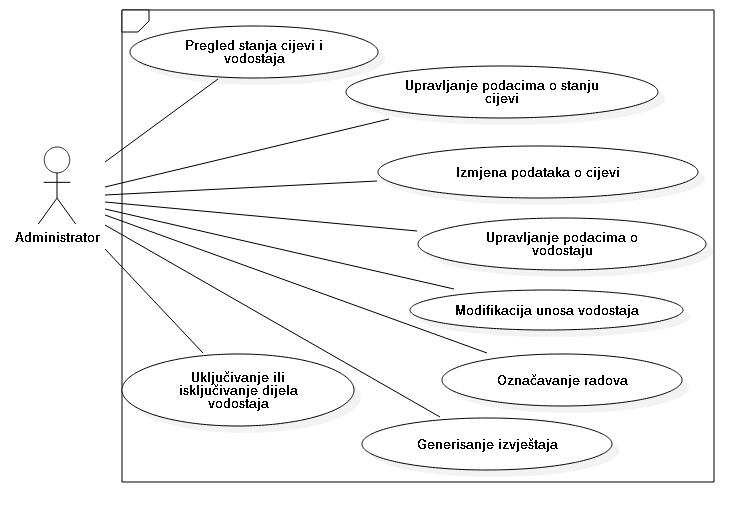
\includegraphics[width=12cm]{uc.png}
\\
\textit{Slika 2:  Dijagram koji pokazuje sve aktivnosti korisnika sa privilegijom Radnik}
\end{center}

\section{Pretpostavke i zavisnosti}

\textbf{Pretpostavka 1.}\\
Pretpostavlja se da nije potrebno vršiti integraciju sa starim sistemom s obzirom  da na istom ne postoji grafički interfejs u vidu vodovodne mape. 
 
 \noindent
\textbf{Pretpostavka 2.}\\
Pretpostavlja se da je serverski računar smješten u prostoriju s fizičkom zaštitom na ulazu i uređajima koji vrše regulaciju temperature koja je preporučena u zvaničnoj dokumentaciji serverske opreme. 

\noindent
\textbf{Pretpostavka 3.}\\
Pretpostavlja se da serverski računar ima stabilno napajanje električnom energijom 24 sata na dan i da postoji UPS uređaj, koji će poslužiti kao rezervna mogućnost u slučaju nepredviđenih okolnosti. 

\noindent
\textbf{Pretpostavka 4.}\\
Prepostavlja se da kompanija ima odgovarajuću mrežnu infrastrukturu, koja će omogućiti da su računari na kojim se izvršava razvijeni softver na ispravan način povezani sa server računarom. 

\noindent
\textbf{Pretpostavka 5.}\\
Pretpostavlja se da korisnici ovog sistema posjeduju osnovno znanje o radu na računaru. 

\noindent
\textbf{Pretpostavka 6.}\\
Pretpostavlja se da će korisnici sistema unositi samo istinite podatke, koji će kasnije biti korišteni u kreiranju izvještaja. 

\noindent
\textbf{Pretpostavka 7.}\\
Pretpostavlja se da će se korisnici sistema odgovorno odnositi prema svojim korisničkim podacima za prijavu na sistem i da iste neće dijeliti s drugim osobama. 

\noindent
\textbf{Pretpostavka 8.}\\
Pretpostavlja se da će korisnici sistema nakon svake prijave na sistem i upotrebe sistema, na ispravan način izvršiti odjavljivanje sa sistema. 

\noindent
\textbf{Pretpostavka 9.}\\
Pretpostavlja se da pristup server računaru s centralnom bazom podataka nema niko drugi osim ovlaštene osobe i da ovlaštena osoba neće zloupotrijebiti svoj položaj i izvršiti manipulacije s podacima u bazi podataka. 
 
\noindent
\textbf{Pretpostavka 10.}\\
Pretpostavlja se da korisnici računara na kojima je instalirana aplikacija imaju ograničene korisničke račune na operativnim sistemima te da im je onemogućeno brisanje sistemskih datoteka,  brisanje datoteka razvijenog softvera i da im je onemogućeno instaliranje drugih softvera. 

\noindent
\textbf{Pretpostavka 11. }\\
Pretpostavlja se da kompanija nalazi unutar prostora Federacije Bosne i Hercegovine, odnosno da je kompanija zajedno s uposlenicima dužna poštovati samo Zakon o radu Federacije Bosne i Hercegovine. 
 

\section{Planiranje zahtjeva}

Zahtjevi koji su opisani u ovom dokumentu nastali su isključivo na osnovu zahtjeva  naručioca sistema, te  navedenih zakonskih regulativa.
\noindent
Ukoliko naručilac sistema zahtijeva promjene specifikacije, tj ukoliko klijent želi napraviti neke promjene u zahtjevima, dodati nove funkcionalnosti, izbaciti stare, potrebno je pratiti sljedeću proceduru: 
\begin{compactitem}
\item Klijent je dužan dostaviti zvanični zahtjev koji detaljno specificira sve promjene koje klijent želi napraviti na sistemu.  Ovaj dokument mora biti potpisan od strane ovlaštene osobe. 
\item Kompanija se obavezuje da će u najkraćem roku, najkasnije 15 dana, napraviti analizu traženih zahtjeva, te će shodno tome klijentu dostaviti odgovor u vidu ponude za nastavak poslovanja koja u zavisnosti od rezultata analize uključuje tražene promjene.  
\item Klijent je dužan nakon toga dostaviti odgovor, nakon čega klijent i kompanija zaključuju novi ugovor, pri čemu se vrši revizija  SRS-a sa novim zahtjevima, koji postaje obavezujući za obje strane. 
\end{compactitem}
 \vspace*{0.25cm}
 \noindent
Prema iznad navedenim stavkama, kompanija zadržava pravo da ne pristane na izvršavanje traženih promjena. Faktori koji mogu uticati na to da kompanija ne prihvati promjene koje klijent zahtjeva su: 
\begin{compactitem}
\item Vremenski period potreban za rješavanje problema 
\item Troškovi potrebni za rješavanje problema 
\item Dostupnost radne snage 
\item Neophodnost zahtjeva 
\end{compactitem}

\vspace*{0.25cm}
\noindent
Ukoliko razvojni tim kompanije uoči potrebu za izmjenama specificiranih zahtjeva klijenta (dodavanje, izmjena ili brisanje zahtjeva) potrebno je pratiti sljedeću proceduru: 
\begin{compactitem}
\item Kompanija je dužna sastaviti Zahtjev za promjenu specifikacije, kojeg potpisuje ovlaštena osoba, i isti dostaviti klijentu. U          zahtevu trebaju biti detaljno opisane sve promjene, te njihov uticaj na sistem. 
\item Klijent je dužan dostaviti odgovor, najkasnije 15 dana od dana prijema Zahtjeva, u kojem se izjašnjava o promjenama. 
\item Ukoliko se klijent složi sa upućenim zahtjevom, vrši se revizija SRS dokumenta, koji tada postaje obavezujući za obje strane.
\end{compactitem}

\chapter{Konkretni zahtjevi}
\section{Vanjski interfejsi}

\subsection{Korisnički interfejsi}
Korisnički interfejs doprinose poboljšanju kvalitete komunikacije sa klijentima i omogućava da korisnici na jednostavan i intuitivan način koriste sve funkcionalnosti sistema. Imamo jednu vrstu korisnika: korisnika sa privilegijama radnika. Naš sistem treba da omogućava  ostvarivanje funkcionalnih zahtjeva koji se mogu grupisati u sljedeće veće cjeline: 
\begin{compactitem}
\item  Pregled karte vodovoda
\item Brisanje i modificiranje podataka o cijevima i vodostaju na karti
\item Generisanje izvještaja 
\end{compactitem}
 U nastavku će biti objašnjeni korisnički interfejsi onim redoslijedom kojim korisnik vrši željene aktivnosti, te su u skladu s tim i numerisani.

\begin{center}
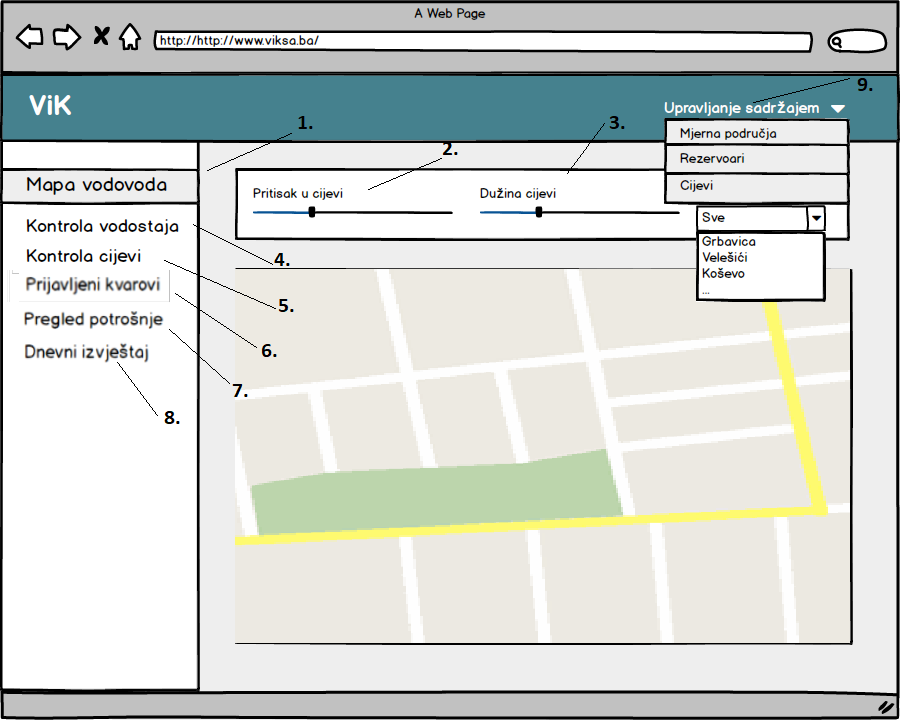
\includegraphics[width=13cm]{UI3.png}
\end{center}

Ovo je izgled početnog ekraja.
\\
\\
1. Klikom na dugme 1 korisniku se prikazuje mapa vodovoda.
\\
\\
2. Prikazuje pritisak u cijevi odabranoj na mapi.
\\
\\
3. Prikazuje dužinu cijevi odabrane na mapi.
\\
\\
4. Klikom na dugme 4 korisniku se prikazuje forma za kontrolu vodostaja.
\\
\\
5. Klikom na dugme 5 korisniku se prikazuje forma za kontrolu cijevi.
\\
\\
6. Klikom na dugme 6 korisniku se prikazuje forma za pregled prijavljenih kvarova.
\\
\\
7. Klikom na dugme 7 korisniku se prikazuje forma za pregled ukupne potrošnje.
\\
\\
8. Klikom na dugme 8 korisniku se prikazuje forma za generisanje izvještaja.
\\
\\
9. Odabirom ove opcije korisniku se nudi mogućnost pregleda i uređivanja detalja o mjernim područjima, rezervoarima i cijevima.

\begin{center}
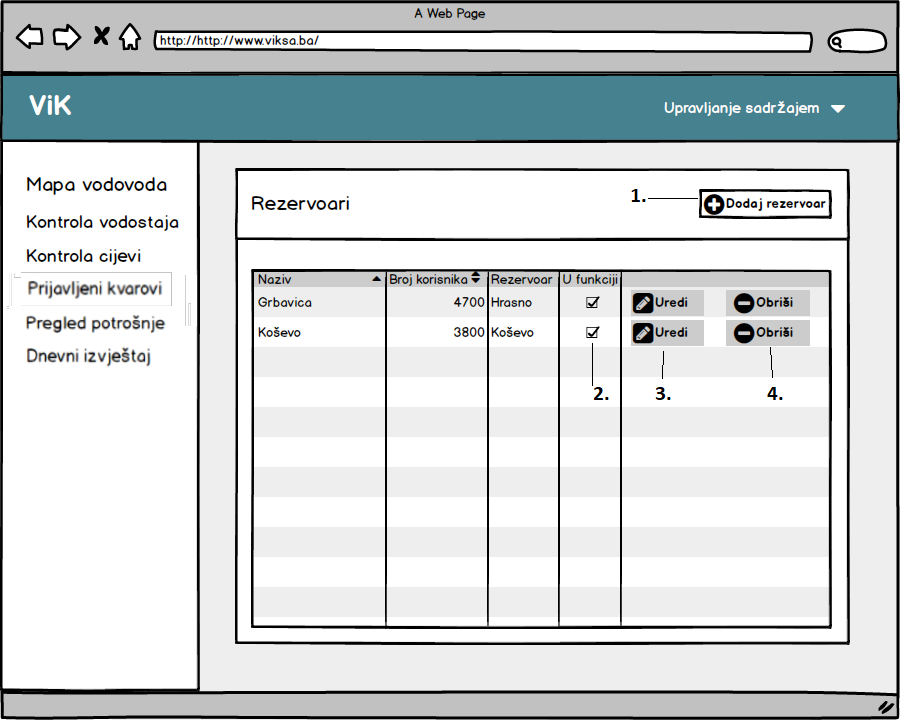
\includegraphics[width=13cm]{UI4.png}
\end{center}

1.Klikom na dugme 1 nudi se mogućnost dodavanja novog rezervoara.
\\
\\
2.Klikom na opciju 2 označava se da li je rezervoar u funkciji ili nije.
\\
\\
3.Klikom na dugme 3 moguće je da se modifikuje postojeći rezervoar.
\\
\\
4.Klikom na dugme 4 moguće je da se obriše postojeći rezervoar.

\begin{center}
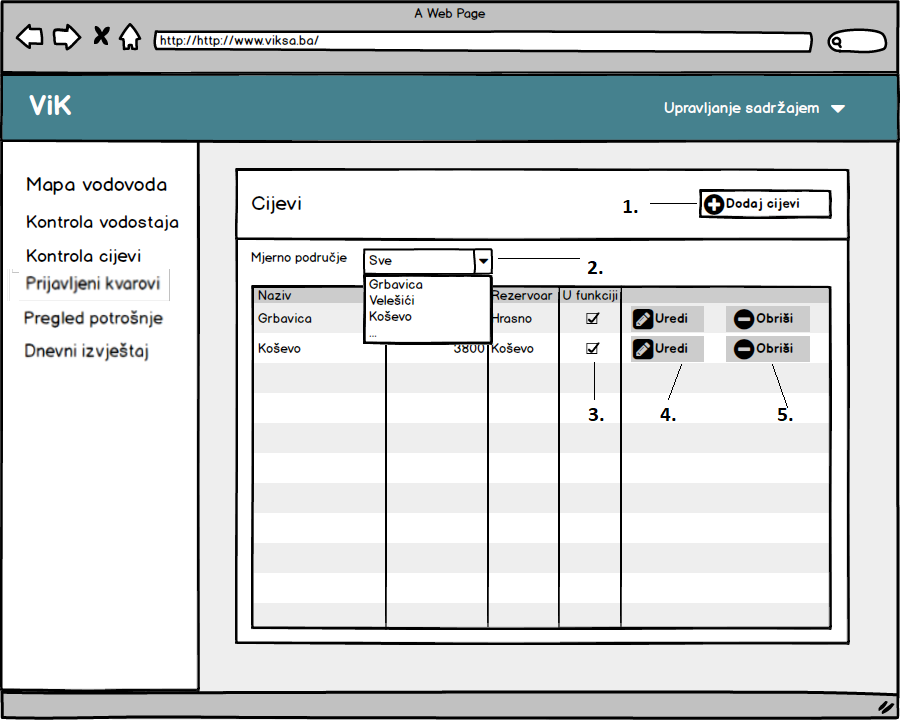
\includegraphics[width=13cm]{UI2.png}
\end{center}

1. Klikom na dugme 1 nodi se mogućnost učitavanja datoteke sa listom cijevi i detalja o njima.
\\
\\
2. Odabirom mjernog područja se filtrira lista cijevi.
\\
\\
3. Označavanje da li je cijev u funkciji ili ne.
\\
\\
4. Klikom na dugme 4 nudi se mogućnost uređivanja detalja o odgovarajućoj cijevi.
\\
\\
5. Klikom na dugme 5 briše se odgovarajuća cijev.

\begin{center}
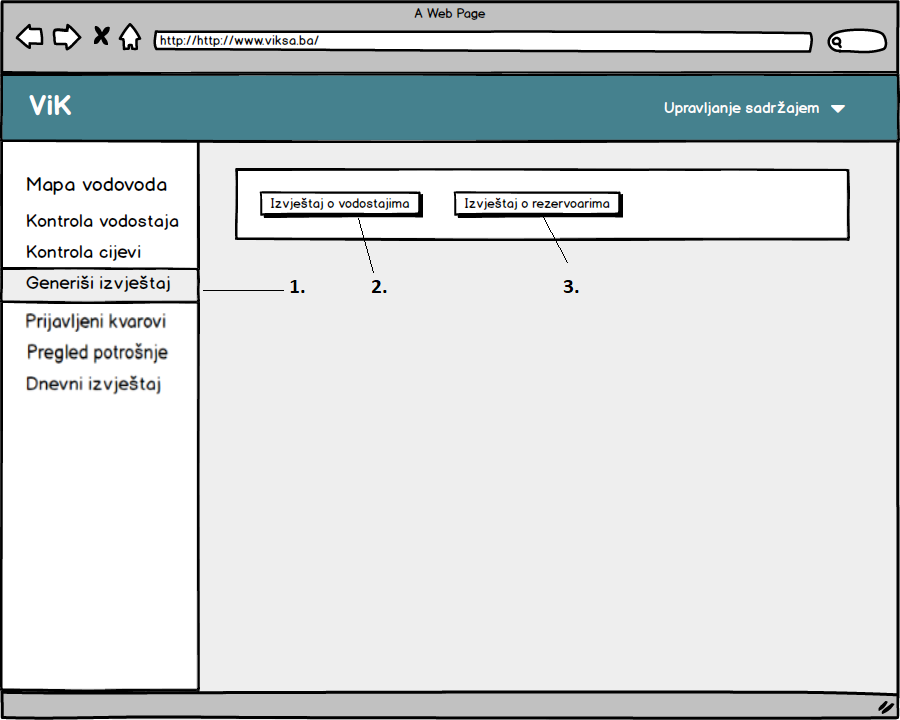
\includegraphics[width=13cm]{UI1.png}
\end{center}

1. Klikom na dugme 1 otvara se forma za generisanje izvještaja
\\\\2. Klikom na dugme 2 generiše se izvještaj o vodostajima, te se u formi .pdf spašava na klijentski uređaj.
\\\\3. Klikom na dugme 3 generiše se izvještaj o rezervoarima, te se u formi .pdf spašava na klijentski uređaj.

\begin{center}
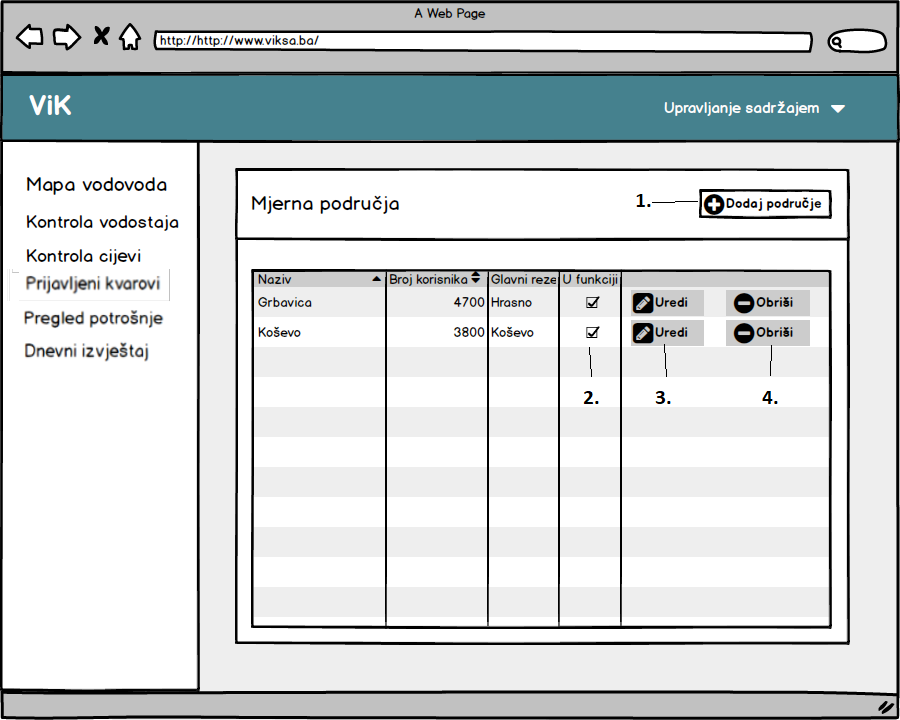
\includegraphics[width=13cm]{UI5.png}
\end{center}

1.Klikom na dugme 1 nudi se mogućnost dodavanja novog područja
\\
\\
2.Klikom na opciju 2 označava se da li je područje u funkciji ili nije
\\
\\
3.Klikom na dugme 3 moguće je da se modifikuje postojeće područje
\\
\\
4.Klikom na dugme 4 moguće je da se obriše postojeće područje
\subsection{Softverski interfejs}
Klijentski dio aplikacije će se moći izvršavati na bilo kojem uređaju sa internet pretraživačem, neovisno o operativnom sistemu. 
  
\subsection{Hardverski i komunikacijski interfejsi}
Hardverski interfejs se sastoji od: monitor, tastatura, miš i printer. Za potrebe printanja izvještaja koristit će se printer koji omogućava printanje dokumenata. Računari su povezani u mrežu preko Ethernet protokola uz korištenje mrežne opreme: routeri, switchevi, mrežni kablovi. Za nesmetano funkcionisanje sistema za pohranu i dobavljanje podataka potrebno je da računari na kojima se koristi aplikacija budu uvezani u mrežu na način da imaju pristup centralizovanoj bazi podataka koja se nalazi na serveru. 


% Ovo su standardne stvari za sistem (Login, administracija nad korisnicima i sl)

\begingroup
\renewcommand{\cleardoublepage}{}
\renewcommand{\clearpage}{}
\section{Funkcionalni zahtjevi}
\endgroup

\subsection{Prikaz mape vodovodne mreže}
  
\begin{tabular}{rp{.95\textwidth}}
Opis &
Korisniku se nakon pristupa web stranici prikazuje mapa vodovodne mreže, na kojoj su prikazane cijevi i vodovodi, te mu se nudi mogućnost odabira većine predviđenih funkcionalnosti upravo preko ove mape.  Ova funcionalnost podliježe Zakonu o vodama Kantona Sarajevo član 22.
\hspace{12pt} 

\\
Preduslovi &
\begin{compactitem}
   \item Zaposlenik je prijavljen na svoj korisnički račun
\end{compactitem}
 
\\
Ulaz &
\begin{compactitem}
   \item Nema ulaza
\end{compactitem}
\\
Uslovi validnosti &
 \begin{compactitem}
   \item Nema uslova validnosti
\end{compactitem}

\\
Procesiranje &
 
\begin{compactitem}
   \item Korisnik ulazi na web stranicu
   \item Korisniku se prikazuje mapa vodovodne mreže
\end{compactitem}
 
\\
Izlaz &
 
\begin{compactitem}
   \item Prikazana mapa vodovodne mreže
   \item Mogućnost odabira drugih funkcionalnosti vezanih za cijevi i vodostaje
\end{compactitem}

\\
Funkcionalni zahtjevi &
 
\begin{compactitem}
  \item FZ 1.1 Sistem omogućava prikaz mape vodovodne mreže 
    \item FZ 1.2 Sistem omogućava interakciju sa mapom kroz ostale funkcionalne zahtjeve
  
\end{compactitem}
 
\\
Prioritet realizacije &
%ovo hspace ostavi za poravnanje%
\hspace{12pt} Visok prioritet

\end{tabular}


%%% COPY OVO ISPOD %%%%

\subsection{Unos podataka o cijevima}
 
\begin{tabular}{rp{.95\textwidth}}
Opis &
Korisnik nakon odabira ove funkcionalnosti unosi podatke o cijevina kao što su mjesto gdje se nalazi, pritisak u cijevi, da li može da predstavlja kritičnu cijev itd.Ova funcionalnost podliježe Zakonu o vodama Kantona Sarajevo član 17.
\hspace{12pt} 

\\
Preduslovi &
\begin{compactitem}
   \item Zaposlenik je prijavljen na svoj korisnički račun
\end{compactitem}
 
\\
Ulaz &
 
\begin{compactitem}
   \item Mjesto gdje se nalazi cijev
   \item Dužina cijevi
   \item Pritisak cijevi
   \item Postoji li mogućnost sa postane kritična cijev
\end{compactitem}
 
\\
Uslovi validnosti &
 
\begin{compactitem}
       \item Uneseni su podaci koji su dozvoljene vrijednosti
\end{compactitem}
 
\\
Procesiranje &
 
\begin{compactitem}
   \item Korisnik odabire cijev kojoj želi unijeti podatke
   \item Korisnik unosi odgovarajuće podatke
   \item Sistem validira unesene podatke
   \item Ukoliko je vrijednost dozvoljena, ažurira se prikaz šeme
\end{compactitem}
 
\\
Izlaz &
 
\begin{compactitem}
   \item Poruka o uspješno ili neuspješno unesenim podacima.
\end{compactitem}
 
\\
Funkcionalni zahtjevi &
 
\begin{compactitem}
  \item FZ 2.1 Sistem omogućava odabir željene cijevi 
    \item FZ 2.2 Sistem omogućava unos podataka/vrijednosti
    \item FZ 2.3 Sistem omogućava validaciju unesene vrijednosti
    \item FZ 2.4 Sistem omogućava prikaz ažurirane šeme
\end{compactitem}
 
\\
Prioritet realizacije &
%ovo hspace ostavi za poravnanje%
\hspace{12pt} Visok prioritet

\end{tabular}
 
%% OVDJE KRAJ SABLONA %%


\newpage % izbaci ako je vec nova, tj napravio je bezveze praznu stranicu


\subsection{Detaljni pregled stanja cijevi}
% Ovo bi valjda bilo kada se klikne jedna cijev na shemi. Detaljni pregled gdje se vide svi podaci za ovu cijev

%%% COPY OVO ISPOD %%%%

\begin{tabular}{rp{.95\textwidth}}
Opis & Nakon odabrane cijevi sa sheme svih cijevi u sistemu, korisnik ima mogućnost detaljnog pregleda svih podataka za odabranu cijev poput mjesta gdje se nalazi cijev, dužine cijevi, pritiska cijevi kao i mogućnost rizika da odabrana cijev postane kritična.Ova funcionalnost podliježe Zakonu o vodama Kantona Sarajevo član 17.
%ovo hspace ostavi za poravnanje%

\\
Preduslovi & 
\begin{compactitem}
    \item Postoje validno uneseni podaci o cijevima
\end{compactitem}

\\
Ulaz & 

\begin{compactitem} 
    \item Nema ulaza
\end{compactitem}

\\
Uslovi validnosti &

\begin{compactitem} 
    \item Nema
\end{compactitem}

\\
Procesiranje &

\begin{compactitem} 
    \item Korisnik ima otvorenu shemu svih cijevi u sistemu
    \item Korisnik odabire željenu cijev za prikaz detalja
    \item Sistem prikazuje sve detalja o odabranoj cijevi
\end{compactitem}

\\
Izlaz &

\begin{compactitem} 
    \item Prikaz svih detalja odabrane cijevi
\end{compactitem}

\\
Funkcionalni zahtjevi &

\begin{compactitem} 
    \item FZ 3.1 Sistem omogućava odabir željene cijevi
    \item FZ 3.2 Sistem omogućava prikaz svih detalja vezanih za odabranu cijev
\end{compactitem}

\\
Prioritet realizacije &
%ovo hspace ostavi za poravnanje%
\hspace{12pt} Visok prioritet
\\
\end{tabular}

%% OVDJE KRAJ SABLONA %%






\subsection{Unos vodostaja}

\begin{tabular}{rp{.95\textwidth}}
Opis & 
%ovo hspace ostavi za poravnanje%
\hspace{12pt} Korisnik označava željeno mjesto za unos vodostaja, te u skladu sa vrijednošću kojom raspolaže ažurira dati podatak u mreži.Ova funcionalnost podliježe Zakonu o vodama Kantona Sarajevo član 17.

\\
Preduslovi & 
\begin{compactitem}
    \item Korisnik ima pristup mreži
\end{compactitem}

\\
Ulaz & 

\begin{compactitem} 
    \item Vrijednost vodostaja
\end{compactitem}

\\
Uslovi validnosti &

\begin{compactitem} 
    \item Izabrano je odgovarajuće mjesto za unos
    \item Vrijednost za unos je u okvirima dozvoljenih vrijednosti
\end{compactitem}

\\
Procesiranje &

\begin{compactitem} 
    \item Korisnik bira odgovarajuće mjesto za unos, te unosi željenu vrijednost
    \item Sistem vrši validaciju vrijednosti
    \item Ukoliko je vrijednost dozvoljena, ažurira se prikaz šeme
\end{compactitem}

\\
Izlaz &

\begin{compactitem} 
    \item Poruka o uspješnom dodavanju vrijednosti
\end{compactitem}

\\
Funkcionalni zahtjevi &

\begin{compactitem} 
    \item FZ 4.1 Sistem omogućava odabir željenog mjesta
    \item FZ 4.2 Sistem omogućava unos korisničkih podataka/vrijednosti
    \item FZ 4.3 Sistem omogućava validaciju unesene vrijednosti
    \item FZ 4.4 Sistem omogućava prikaz ažurirane šeme
\end{compactitem}

\\
Prioritet realizacije &
%ovo hspace ostavi za poravnanje%
\hspace{12pt} 
Visok prioritet
\end{tabular}


\newpage % izbaci ako je vec nova, tj napravio je bezveze praznu stranicu
\subsection{Kreiranje izvještaja}
%%% COPY OVO ISPOD %%%%

\begin{tabular}{rp{.95\textwidth}}
Opis & 
%ovo hspace ostavi za poravnanje%
\hspace{12pt} Nakon odabira opcije za kreiranje izvještaja, kreira se izvještaj koji je sastavljen od svih aktivnosti koje su u toku dana urađene na sistemu.

\\
Preduslovi & 
\begin{compactitem}
    \item Zaposlenik je prijavljen na svoj korisnički račun  
\end{compactitem}

\\
Ulaz &
 
\begin{compactitem}
   \item Nema ulaza
\end{compactitem}
 
\\
Uslovi validnosti &
 
\begin{compactitem}
       \item Nema uslova validnosti
\end{compactitem}
\\


\\
Procesiranje &

\begin{compactitem} 
    \item Kokisnik odabere opciju za kreiranje izvještaja
    \item Sistem kreira izvještaj
\end{compactitem}

\\
Izlaz &

\begin{compactitem} 
    \item Pregled izvještaja o svim aktivnostima na sistemu u toku dana
\end{compactitem}

\\
Funkcionalni zahtjevi &

\begin{compactitem} 
    \item FZ 5.1 Sistem omogućava odabir kreiranja izvještaja
    \item FZ 5.2 Sistem omogućava prikaz izvještaja
    \item FZ 5.3. Sistem omogućava printanje izvještaja
\end{compactitem}

\\
Prioritet realizacije &
%ovo hspace ostavi za poravnanje%
\hspace{12pt} Nizak prioritet
\\
\end{tabular}

%% OVDJE KRAJ SABLONA %%


% izbaci ako je vec nova, tj napravio je bezveze praznu stranicu
\subsection{Označavanje radova}

%%% COPY OVO ISPOD %%%%

\begin{tabular}{rp{.95\textwidth}}
Opis & 
%ovo hspace ostavi za poravnanje%
\hspace{12pt} Sistem će omogučiti registraciju radova unutar mreže.Ova funcionalnost podliježe Zakonu o vodama Kantona Sarajevo član 17.

\\
Preduslovi & 
\begin{compactitem}
    \item U sistemu je registrovana barem jedna cijev
\end{compactitem}

\\
Ulaz & 

\begin{compactitem} 
    \item Cijev unutar mreže
\end{compactitem}

\\
Uslovi validnosti &

\begin{compactitem} 
    \item Ulazni podatak nije prazan
    \item Ne postoje već postojeći radovi na odabranoj cijevi
\end{compactitem}

\\
Procesiranje &

\begin{compactitem} 
    \item Korisnik bira odgovarajuću opciju nad cijevi na šemi
    \item Sistem registruje radove nad cijevi unutar sistema
\end{compactitem}

\\
Izlaz &

\begin{compactitem} 
    \item Poruka o uspješno izvršenoj akciji
\end{compactitem}

\\
Funkcionalni zahtjevi &

\begin{compactitem} 
    \item FZ 6.1 Prikaz vodovodne mreže
    \item FZ 6.2 Odabir jedne cijevi na mreži
    \item FZ 6.3 Podrška za pohranu radova unutar baze podataka
\end{compactitem}

\\
Prioritet realizacije &
%ovo hspace ostavi za poravnanje%
\hspace{12pt} Srednje visok prioritet
\end{tabular}

%% OVDJE KRAJ SABLONA %%

\subsection{Isključivanje dijela vodovoda}
\begin{tabular}{rp{.5\textwidth}}
Opis & 
%ovo hspace ostavi za poravnanje%
\hspace{12pt} Korisnik će imati mogućnost isključivanja željenih dijelova vodovoda. Ovo podrazumijeva da je vodovodna mreža koja je prikazana na mapi podijeljena na određene dijelove. Na mapi je prikazana mapa jednog područja, gdje dijelovi predstavljaju sva naselja priključena na vodovodnu mrežu. U okviru svakog dijela vodovodne mreže postoji ikona ventila. Klikom na tu ikonu korisniku se nudi mogućnost iključenja tog određenog dijela iz vodovodne mreže. Svi isključeni dijelovi su obojeni sivom bojom.Ova funcionalnost podliježe Zakonu o vodama Kantona Sarajevo član 22.
\\
Preduslovi & 
\begin{compactitem}
    \item Korisnik je prijavljen na sistem
    \item Dio koji se želi isključiti je priključen na vodovodnu mrežu
\end{compactitem}

\\
Ulaz & 

\begin{compactitem} 
      \item Nema ulaza
    \end{compactitem}

\\
Uslovi validnosti &

\begin{compactitem} 
   \item  Dio koji se želi isključiti je priključen na vodovodnu mrežu
\end{compactitem}

\\
Procesiranje &

\begin{compactitem} 
    \item Korisnik vrši odabir dijela mreže koji želi isključiti
    \item Klikom na ikonu ventila korisniku se nudi opcija isključivanja dijela vodovodne mreže
    \item Isključeni dio se obilježava sivom bojom

\end{compactitem}

\\
Izlaz &

\begin{compactitem} 
    \item Poruka o uspješnom isključivanju dijela mreže
\end{compactitem}

\\
Funkcionalni zahtjevi &

\begin{compactitem} 
    \item FZ 7.1 Prikaz vodovodne mreže
    \item FZ 7.2 Isključivanje dijela vodovoda
\end{compactitem}

\\
Prioritet realizacije &
%ovo hspace ostavi za poravnanje%
\hspace{12pt} Srednje visok prioritet
\\
\end{tabular}

\newpage 

\subsection{Uključivanje dijela vodovoda}
\begin{tabular}{rp{.5\textwidth}}
Opis & 
%ovo hspace ostavi za poravnanje%
\hspace{12pt} Korisnik će imati mogućnost uključivanja željenih dijelova vodovoda, koji su već isključeni. U okviru svakog dijela vodovodne mreže postoji ikona ventila. Klikom na tu ikonu korisniku se nudi mogućnost uključenja određenog dijela iz vodovodne mreže. Ova funcionalnost podliježe Zakonu o vodama Kantona Sarajevo član 22.

\\
Preduslovi & 
\begin{compactitem}
    \item Korisnik je prijavljen na sistem
    \item Dio koji se želi uključiti je isključen iz vodovodne mreže
\end{compactitem}

\\
Ulaz & 

\begin{compactitem} 
      \item Nema ulaza
    \end{compactitem}

\\
Uslovi validnosti &

\begin{compactitem} 
   \item  Dio koji se želi uključiti je isključen iz vodovodne mreže
\end{compactitem}

\\
Procesiranje &

\begin{compactitem} 
    \item Korisnik vrši odabir dijela mreže koji želi uključiti
    \item Klikom na ikonu ventila korisniku se nudi opcija uključivanja dijela vodovodne mreže

\end{compactitem}

\\
Izlaz &

\begin{compactitem} 
    \item Poruka o uspješnom uključivanju dijela mreže
\end{compactitem}

\\
Funkcionalni zahtjevi &

\begin{compactitem} 
    \item 8.1 Prikaz vodovodne mreže
    \item 8.2 Uključivanje dijela vodovoda
\end{compactitem}

\\
Prioritet realizacije &
%ovo hspace ostavi za poravnanje%
\hspace{12pt} Srednje visok prioritet
\\
\end{tabular}


%% OVDJE KRAJ SABLONA %%

\newpage

\section{Nefunkcionalni zahtjevi i osobine sistema}
\subsection{Upotrebljivost sistema}

Sistem će posjedovati vrlo intuitivan grafički interfejs što će zahtjevati vrlo malo truda pri njegovom korištenju, ali u isto vrijeme biti vrlo efikasan za postizanje svog cilja. Budući da je sistem prije svega dizajniran za korisnike za koji ne moraju  imati visoko informatičko znanje, potrebno je obezbijediti odgovarajuće upute svim korisnicima. Uzimajući to u obzir, nameću se sljedeći nefunkcionalni zahtjevi: 
 
\begin{compactitem}
\item \textbf{NFZ 1:} Korisnički interfejs mora biti na bosanskom jeziku. \vspace*{0.1cm}
 
\item \textbf{NFZ 2:} Korisnički interfejs mora biti jednostavan i intuitivan, bez suvišnih detalja i dodatnih prozora. \vspace*{0.1cm}
 
\item \textbf{NFZ 3:} Korisnički interfejs treba sadržavati što manje linkova. \vspace*{0.1cm}
 
\item \textbf{NFZ 4:} Fontovi, kao i njihova veličina moraju biti prilagođeni za maksimalnu čitljivost. \vspace*{0.1cm}
 
\item \textbf{NFZ 5:} Korisnički interfejs treba biti dizajniran tako da korisnicima pruža pomoć pri njegovom korištenju.  \vspace*{0.1cm}
 
\item \textbf{NFZ 6:} Korisniku će biti pruženo objašnjenje za svaku komponentu interfejsa koje će sadržavati njegovu svrhu i upute pri njenom korištenju. \vspace*{0.1cm}
\end{compactitem}

\subsection{Perfomanse sistema}

Pošto performanse sistema zavise od brzine internet konekcije, uzima se u obzir da je brzina internet konekcije prosječna brzina internet konekcije u BiH, tj 10Mb/s. Veća brzina internet konkecije može, ali nužno ne mora rezultirati boljim performansama sistema.

\subsection{Atributi kvaliteta sistema}

\subsection{Fizička sigurnost sistema}

Kompaniji nije u opisu posla da provjerava da li su zadovoljeni uvjeti fizičke sigurnosti.

\subsection{Sigurnost sistema}

\begin{compactitem}

\item \textbf{NFZ 7} Sistem će imati kontrolu pristupa čime se svakom korisniku dozvoljava pristup samo onim funkcionalnostima koji su mu dodjeljeni.
\vspace*{0.5cm}
\item \textbf{NZF 8} Pristupni podaci će se automatski generisati za svakog korisnika, a iste će se izmjeniti prilikom prvog pristupa sistemu od strane korisnika.

\end{compactitem}

\subsection{Backup}
\begin{compactitem} 
% Potrebno je jos uvrstiti tacne brojeve ovdje kod NFZ, a to nije moguce dok se sve iznad ne napise...
    \item \textbf{NFZ 9} Diskovi na kojima se nalazi baza podataka, kao i diskovi na kojima je web aplikacija, će biti podešeni u RAID1 šemi što obezbjeđuje backup u slučaju fizičkog ispada jednog diska, kao i momentalnu upotrebu istog. 
    \vspace*{0.2cm}
    \item \textbf{NFZ 10} Web aplikacija je sama po sebi statična, pa će se njen backup vršiti za svaku novu verziju prilikom same instalacije.
    \vspace*{0.2cm}
    \item \textbf{NFZ 11} Baza podataka će se automatski (svake nedjelje tokom neradnih večernjih sati) smjestiti na eksterni  SFTP server.
\end{compactitem}

\subsection{Portabilnost sistema}

\begin{compactitem}
\item \textbf{NFZ 12} Sa obzirom da se radi o web aplikaciji, sistemu je moguće pristupiti sa bilo kojeg uređaja sa internet pristupom i odgovarajućim internet pretraživačem.
\end{compactitem}

\subsection{Skalabilnost sistema}

\begin{compactitem}

\item \textbf{NFZ 13} Modularni dizajn sistema će omogućiti proširivanje mreže (dodavanjem novih cijevi) i dodavanje novih senzora kroz administrativni panel sistema. Broj korisnika, cijevi i senzora nije ograničen, te povećanje istih ne utiče na vrijeme odziva sistema.

\end{compactitem}

\subsection{Dostupnost}

\begin{compactitem}
\item \textbf{NFZ 14} Sistem će biti dostupan 24 sata dnevno, 7 dana u sedmici. Izuzeci su eventualni nepredviđeni kvarovi.
\end{compactitem}

\subsection{Održavanje sistema}

\begin{compactitem}
\item \textbf{NFZ 15} Omogućit će se nadogradnja softvera u periodu izvan radnog vremena.

\end{compactitem}


\end{document}



